\begin{figure}[tbp]
  \centering
  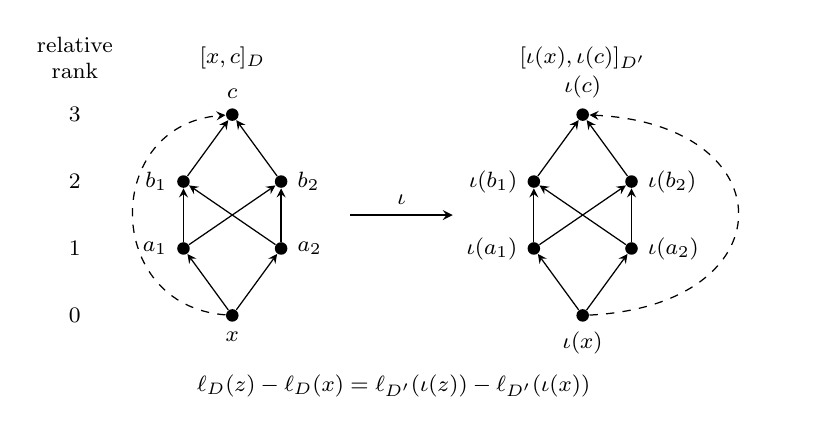
\begin{tikzpicture}[
    x=1cm,y=.85cm,
    font=\footnotesize,
    vertex/.style={circle,fill=black,inner sep=1.6pt},
    cover/.style={->,>=stealth,line width=.45pt},
    longedge/.style={cover,dashed},
    every label/.style={font=\footnotesize}
  ]
    \node[align=center] at (-2.0,3.85) {relative\\rank};
    \foreach \r in {0,1,2,3}
      \node at (-2.0,\r) {$\r$};

    \node at (0,3.85) {$[x,c]_D$};
    \node[vertex,label=below:$x$] (x) at (0,0) {};
    \node[vertex,label=left:$a_1$] (a1) at (-.62,1) {};
    \node[vertex,label=right:$a_2$] (a2) at (.62,1) {};
    \node[vertex,label=left:$b_1$] (b1) at (-.62,2) {};
    \node[vertex,label=right:$b_2$] (b2) at (.62,2) {};
    \node[vertex,label=above:$c$] (c) at (0,3) {};
    \draw[cover] (x)--(a1);
    \draw[cover] (x)--(a2);
    \draw[cover] (a1)--(b1);
    \draw[cover] (a1)--(b2);
    \draw[cover] (a2)--(b1);
    \draw[cover] (a2)--(b2);
    \draw[cover] (b1)--(c);
    \draw[cover] (b2)--(c);
    \draw[longedge] (x) .. controls (-1.65,.15) and (-1.65,2.85) .. (c);

    \begin{scope}[xshift=4.45cm]
      \node at (0,3.85) {$[\iota(x),\iota(c)]_{D'}$};
      \node[vertex,label=below:$\iota(x)$] (ix) at (0,0) {};
      \node[vertex,label=left:$\iota(a_1)$] (ia1) at (-.62,1) {};
      \node[vertex,label=right:$\iota(a_2)$] (ia2) at (.62,1) {};
      \node[vertex,label=left:$\iota(b_1)$] (ib1) at (-.62,2) {};
      \node[vertex,label=right:$\iota(b_2)$] (ib2) at (.62,2) {};
      \node[vertex,label=above:$\iota(c)$] (ic) at (0,3) {};
      \draw[cover] (ix)--(ia1);
      \draw[cover] (ix)--(ia2);
      \draw[cover] (ia1)--(ib1);
      \draw[cover] (ia1)--(ib2);
      \draw[cover] (ia2)--(ib1);
      \draw[cover] (ia2)--(ib2);
      \draw[cover] (ib1)--(ic);
      \draw[cover] (ib2)--(ic);
      \draw[longedge] (ix) .. controls (2.6,.15) and (2.6,2.85) .. (ic);
    \end{scope}

    \draw[->,>=stealth,line width=.6pt]
      (1.5,1.5)--node[above] {$\iota$} (2.8,1.5);
    \node[align=center] at (2.05,-1.05)
      {$\ell_D(z)-\ell_D(x)
        =\ell_{D'}(\iota(z))-\ell_{D'}(\iota(x))$};
  \end{tikzpicture}
  \caption{Transport of a relative dihedral interval of rank three.
    Each internal relative rank contains two vertices.
    The eight solid relative covers give the rank-three instance of the
    closure rule in Theorem~\ref{bg:graph}; the dashed arrow is the recovered
    reflection edge.
    The heights record relative rank differences, not ambient length
    differences, and a relative cover need not be an ambient cover.
    The restriction of $\iota$ preserves these ranks and directed edges;
    no matching of root labels is asserted.}
  \label{fig:dihedral-transport}
\end{figure}
